
\documentclass{vgtc}                          % final (conference style)
%\documentclass[review]{vgtc}                 % review
%\documentclass[widereview]{vgtc}             % wide-spaced review
%\documentclass[preprint]{vgtc}               % preprint
%\documentclass[electronic]{vgtc}             % electronic version

%\usepackage{mathptmx}
\usepackage{graphicx}
\usepackage{times}
\usepackage{url}
\usepackage{epsfig}
\usepackage{psfrag}
\usepackage{amsmath}
\usepackage{amssymb}

%% We encourage the use of mathptmx for consistent usage of times font
%% throughout the proceedings. However, if you encounter conflicts
%% with other math-related packages, you may want to disable it.

%% If you are submitting a paper to a conference for review with a double
%% blind reviewing process, please replace the value ``0'' below with your
%% OnlineID. Otherwise, you may safely leave it at ``0''.
\onlineid{0}

%% declare the category of your paper, only shown in review mode
\vgtccategory{Research}

%% allow for this line if you want the electronic option to work properly
\vgtcinsertpkg

%% In preprint mode you may define your own headline.
%\preprinttext{To appear in an IEEE VGTC sponsored conference.}

%% Paper title.

\title{Interactive Coverage Effectiveness Multiplots For Analyzing \\ Prioritized Regression Test Suites }

%% Author and Affiliation (multiple authors with single affiliations).
%%\author{Roy G. Biv\thanks{e-mail: roy.g.biv@aol.com} %
%%\and Ed Grimley\thanks{e-mail:ed.grimley@aol.com} %
%%\and Martha Stewart\thanks{e-mail:martha.stewart@marthastewart.com}}
%%\affiliation{\scriptsize Martha Stewart Enterprises \\ Microsoft Research}

%%% Author and Affiliation (multiple authors with same affiliation)
%\author{Adam M. Smith\thanks{e-mail: ams292@cs.pitt.edu} %
%\and Joshua J. Geiger\thanks{e-mail:jj55@cs.pitt.edu}} %
%\affiliation{\scriptsize University of Pittsburgh}

%             ORDER?????

%%% many authors and many affiliations
\author{Adam M. Smith\thanks{e-mail: ams292@.cs.pitt.edu}\\ %
  \scriptsize University of Pittsburgh %
\and Joshua J. Geiger \thanks{e-mail:jjg55@cs.pitt.edu}\\ %
     \scriptsize University of Pittsburgh %
\and G. Elisabeta Marai\thanks{e-mail:marai@cs.pitt.edu}\\ %
     \scriptsize University of Pittsburgh %
 \and Gregory M. Kapfhammer\thanks{gkapfham@allegheny.edu} \\ %    
     \scriptsize Allegheny College%
  \and Manos Renieris\thanks{email:manos@google.com} \\
     \scriptsize Google}



\abstract{Software testing increases confidence in the correctness of an application's source code.  Altering a test suite's execution order enables earlier detection of defects and allows developers to fix errors sooner.  The many existing ordering methods produce different possible test suite orders to choose from.  This paper presents tool support for a technique that allows for a comparison of test suite orders through visualization and interaction.}

%% ACM Computing Classification System (CCS). 
%% See <http://www.acm.org/class/1998/> for details.
%% The ``\CCScat'' command takes four arguments.

%%\CCScatlist{ 
 %% \CCScat{K.6.1}{Management of Computing and Information Systems}%
%%{Project and People Management}{Life Cycle};
%%  \CCScat{K.7.m}{The Computing Profession}{Miscellaneous}{Ethics}
%%}

%% Copyright space is enabled by default as required by guidelines.
%% It is disabled by the 'review' option or via the following command:
% \nocopyrightspace

%%%%%%%%%%%%%%%%%%%%%%%%%%%%%%%%%%%%%%%%%%%%%%%%%%%%%%%%%%%%%%%%
%%%%%%%%%%%%%%%%%%%%%% START OF THE PAPER %%%%%%%%%%%%%%%%%%%%%%
%%%%%%%%%%%%%%%%%%%%%%%%%%%%%%%%%%%%%%%%%%%%%%%%%%%%%%%%%%%%%%%%%

\begin{document}

%% The ``\maketitle'' command must be the first command after the
%% ``\begin{document}'' command. It prepares and prints the title block.

%% the only exception to this rule is the \firstsection command
\firstsection{Introduction}

\maketitle

%% \section{Introduction} 

Developers inevitably create errors while designing and implementing software systems. Software developers execute tests $\langle t_1, t_2, t_3,\ldots, t_n\rangle$ in a test suite $T$ to isolate defects and gain confidence in the correctness of the code.  Each test case in the test suite exercises specific points in the system, comparing the actual output of the code to the hand computed expected one.  If a test fails then it is likely that a defect is present in the source code that the test executes.  As the source code grows in size and number of features new tests are written as well.  To ensure that the new features do not cause the system to regress, developers include every previously written test in the collection of tests.  This process of executing and re-executing the entire test suite is known as regression testing.  

Gradually, the addition of new tests increases the size of the test suite until its execution time may become prohibitively expensive.  One method of altering the test suite to resolve this issue is test suite prioritization \cite{rothermelprioritizing2001}.  Prioritization attempts to find an ordering of the test cases that is more likely to locate defaults earlier in the execution of the test suite without risking the loss of coverage by removing a test.  The tests are ordered based on criteria that are obtained during a process called coverage monitoring.  

Coverage monitoring measures and enumerates the specific points in the source code that are executed when a test $t_i$ is run, whether they are a line, a block, a method, a branch \cite{zhu}, or another type.  Each unit of measured code coverage is called a \textit{requirement}.  Given a test suite $T$, coverage monitoring gives a set of requirements $\mathcal{R}(T) = \{ r_1, r_2,\ldots,r_m \}$.  Each individual test $t_i$ is associated with a subset of requirements $\mathcal{R}(t_i) \subseteq \mathcal{R}(T)$, which it is said to \textit{cover}.  

Table \ref{fig:example} shows an example of a test suite with 4 tests and 5 requirements.  An X in a cell $(t_i, r_j)$ represents that $t_i$ covers $r_j$.  Consider running the shown test suite in its original order.  In this case all of the requirements are not covered until 8 time units have passed.  Conversely, if the test suite is executed in reverse order all of the requirements are covered in 4 time units.  Covering all of the requirements sooner allows for a higher chance to find faults earlier so that developers can more quickly begin to make corrections.

The metric coverage effectiveness (CE) \cite{ce} rates a test suite order based on how fast it covers every requirement.  Each test suite offers the possibility of covering more total requirements and when the cumulative coverage is plotted against time a step function is formed as shown in Figure \ref{fig:ce}.  CE is calculated by dividing the area under the step function for the actual order by the area under the curve of the ideal test suite that covers all of its requirements instantly.  This value is inclusively between 0 and 1 where a CE of 0 would mean that no requirements were covered and a CE of 1 would mean that all of the requirements were covered instantly.
%Example Test Suite
\begin{table}[t]
\centering
\begin{tabular}{|c|c|c|c|c|c||c|}
\hline
& $r_1$ & $$ & $r_2$ & $r_3$ & $r_4$ & Execution Time \\
\hline
\hline
$t_1$ & X & X & X & X &     & 4 \\
\hline
$t_2$ &     &    & X & X &     & 1 \\
\hline
$t_3$ &     & X &    &     &     & 1 \\
\hline
$t_4$ & X &    &     &     & X & 2 \\
\hline
\end{tabular}
\vspace{-.1in}
\caption{Example Test Suite}

\vspace{-.15in}

\end{table}
\label{fig:example}

% Coverage Effectiveness
\begin{figure}[t]
\centering
\psfrag{tone1059}[cc][cc]{$t_1$ Done}
\psfrag{tone1060}[cc][cc]{$t_{n-1}$ Done}
\psfrag{tone1061}[cc][cc]{$t_{n}$ Done}
\psfrag{cover1059}[cc][cc]{$\;\;$ Cover $\cal{R}$$(t_1)$}
\psfrag{cover1060}[cc][cc]{Cover $\bigcup_{i = 1}^{n-1}$$ \cal{R}$$(t_i)$}
\psfrag{cover1061}[cc][cc]{\hspace{10pt} Cover $\cal{R}$$(T)$}
\psfrag{area1061}[cc][cc]{\hspace{10pt} Area $\int_0^{l(n)} \mathrm{C}(T, l)$}
\psfrag{ccTc}[cc][cc]{${\scriptstyle \mathrm{C}(T,l)}$}
\psfrag{ttTt}[cc][cc]{$(l)$}

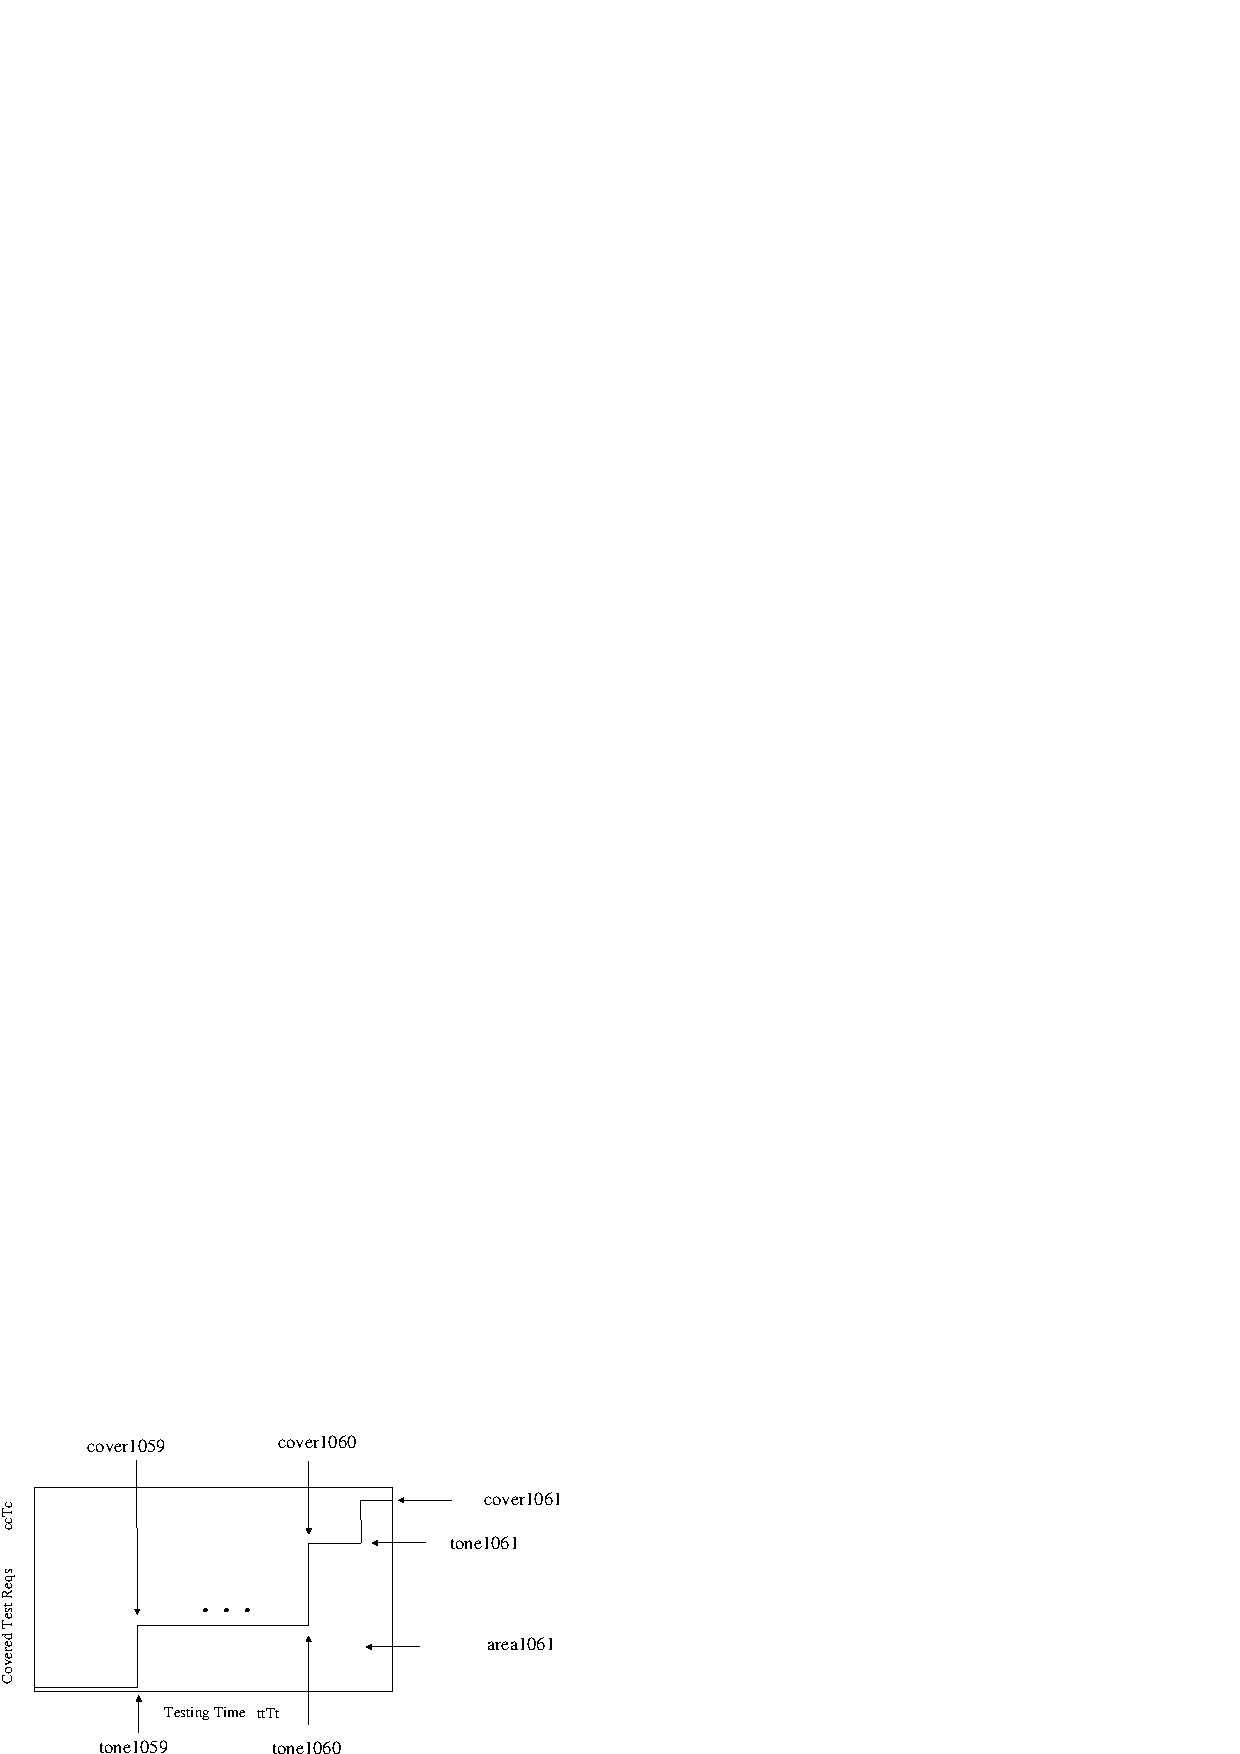
\includegraphics[width=3in]{cum_cov_final.png}
\vspace{-.2in}
\caption{Coverage Effectiveness.} %\cite{ce} (Used with permission of author).} % can't cite in captions apparently.
\vspace{-.25in}
\label{fig:ce}
\end{figure}	

\section{Motivation}

For test suites with $n$ tests it is too expensive to generate all $n\!$ possible orderings to find the best CE value.  For this reason there are several algorithms that prioritize test suites.  Given coverage and timing data for a test suite the tool support for the presented visualization generates several prioritizations using the implementations of greedy (GRD), 2-optimal greedy (2OPT), delayed greedy (DGR), and Harrold Gupta Soffa (HGS) algorithms described by Smith and Kapfhammer \cite{smith:2009}.  These algorithms can use the execution time (cost), covered requirements (coverage), or a ratio of covered requirements per unit time (ratio) to make all necessary greedy choices.

In addition to algorithmic approaches to prioritization, random sampling may produce orderings that are favored over the original order.  Generating large random samples also gives insight into the distribution of CE values across many different orderings of a test suite.  As shown by ***Need to find  citation*** the reverse order of a test suite also tends to produce higher CE values than the original and thus is included in this visualization technique. %need to cite rothermel i think. \cite{{} 

It is difficult to interpret the results of several algorithms or random samples by reading text alone.  Therefore, this paper presents a visualization technique that can allow software testers to view the cumulative coverage and CE of a large set of test suite orders simultaneously.   Related work in the field of visualizing test suites exists \cite{tarantula}, however, it focuses on fault localization or different features of a test suite.  Examining the CE functions of several orderings for a given test suite will quickly reveal the effectiveness of the different prioritization techniques on that test suite.  Figure \ref{fig:multi_ce} shows a multiplot of CE functions for 50 random prioritizations.  This static image does not allow for easy identification of the source of the prioritizations.  Also, the static image cannot display qualitative data without using a large legend.  

\begin{figure}[t]
\centering
\includegraphics[scale=.25]{original.png}
\vspace{-.2in}
\caption{Coverage Effectiveness Multiplot}
\vspace{-.2in}
\end{figure}
\label{fig:multi_ce}

\section{Tool Design}

This visualization technique aids in analyzing multiple prioritizations of a test suite through interactive CE multiplots.  Drawing from characteristics shown by Becker et al$.$ \cite{Stephen95visualizingnetwork} and a NY Times interactive visualization of market statstics \footnote[1]{http://www.nytimes.com/interactive/2008/10/11/business/20081011$\_$BEARMARKETS.html} the tool allows users to interactively select techniques displayed and directly manipulate the corresponding plot.  Data on demand obviates any need for keys or legends.  Figure \ref{fig:screenshot} provides a screen capture of the tool.  

The left panel provides information about the test suite and allows the user to select which technique's results will be displayed in the multiplot.  The first set of buttons will display the original or the reverse order of the test suite.  The button matrix toggles displaying the results of the prioritization algorithms introduced above.  Each row represents a prioritization technique and each column shows a greedy choice metric.  To display the results of a technique given a specific metric the user may click on the appropriate cell in the matrix.  Each technique button is color coded to match its step function line in the plot for easy identification.  The slider bar allows the user to choose a number of random prioritizations that are displayed in the plot as thin gray lines.  Below the slider bar the average CE and standard deviation of CE are displayed for the current sample and also for the entire collection of random priortizations sampled so far.

The right panel displays the multiplot.   The $y$ axis displays the number of requirements and the $x$ axis shows the execution time.  The step functions for the cumulative coverage of the chosen test orderings are plotted in this area.  In Figure \ref{fig:screenshot} all techniques are currently selected to appear in the multiplot.  A mouse-over on a function line highlights it and shades the area under it, as well as provides a label identifying the technique, greedy choice metric, and the CE value of the prioritization represented by the line.    

\section{Evaluation}

 The tool support for this regression test suite visualization technique is available for download at \textit{raise.googlecode.com}.
 
\begin{figure}
\includegraphics[scale=.25]{screenshot.png}
\vspace{-.3in}
\caption{Interactive Coverage Effectiveness Multiplot}
\vspace{-.2in}
\label{fig:screenshot}
\end{figure}

%% if specified like this the section will be ommitted in review mode
%\acknowledgements{}

\bibliographystyle{abbrv}
%%use following if all content of bibtex file should be shown
%\nocite{*}
\bibliography{myBibtexDB}
\end{document}
